% Тут используется класс, установленный на сервере Papeeria. На случай, если
% текст понадобится редактировать где-то в другом месте, рядом лежит файл matmex-diploma-custom.cls
% который в момент своего создания был идентичен классу, установленному на сервере.
% Для того, чтобы им воспользоваться, замените matmex-diploma на matmex-diploma-custom
% Если вы работаете исключительно в Papeeria то мы настоятельно рекомендуем пользоваться
% классом matmex-diploma, поскольку он будет автоматически обновляться по мере внесения корректив
%

% По умолчанию используется шрифт 14 размера. Если нужен 12-й шрифт, уберите опцию [14pt]
% \documentclass[14pt]{matmex-diploma}
\documentclass[14pt]{matmex-diploma-custom}
\usepackage{amsmath}
\usepackage{amssymb}

\begin{document}
% Год, город, название университета и факультета предопределены,
% но можно и поменять.
% Если англоязычная титульная страница не нужна, то ее можно просто удалить.
\filltitle{ru}{
    chair              = {Математическое обеспечение и администрирование информационных систем\\ Кафедра информационно-аналитический систем},
    title              = {Суммаризация групп в социальных сетях},
    % Здесь указывается тип работы. Возможные значения:
    %   coursework - Курсовая работа
    %   diploma - Диплом специалиста
    %   master - Диплом магистра
    %   bachelor - Диплом бакалавра
    type               = {master},
    position           = {студента},
    group              = 646,
    author             = {Чуриков Никита Сергеевич},
    supervisorPosition = {к.\,ф.-м.\,н., доцент},
    supervisor         = {Графеева Н.\,Г.},
    reviewerPosition   = {Директор департамента управления информационными потоками},
    reviewer           = {Яковлев П.\,А.},
    % chairHeadPosition  = {д.\,ф.-м.\,н., профессор},
    % chairHead          = {Хунта К.\,Х.},
%   university         = {Санкт-Петербургский Государственный Университет},
%   faculty            = {Математико-механический факультет},
%   city               = {Санкт-Петербург},
%   year               = {2013}
}
\filltitle{en}{
    chair              = {Software and Administration of Information Systems \\ Sub-Department of Analytical Information System},
    title              = {News resources summarization in social networks},
    author             = {Nikita Churikov},
    supervisorPosition = {Assistant Professor},
    supervisor         = {Natalia Grafeeva},
    reviewerPosition   = {Director of information flow department},
    reviewer           = {Pavel Yakovlev},
    % chairHeadPosition  = {professor},
    % chairHead          = {Christobal Junta},
}
\maketitle
\tableofcontents
% У введения нет номера главы
% \section*{Аннотация}
% Одной из задач обработки естественного языка является задача суммаризации текста.
% Ее целью является уменьшение размера исходного текста без потери ключевой информации.
% В данной работе мы решаем схожую проблему, но для информационных ресурсов в социальных сетях.
% В частности, мы рассматриваем задачи генерации заголовков и выделения ключевых слов,
% поскольку тексты бывают разного объема и потому их можно сжимать разными способами.
% В тексте мы приводим численное обоснование выбранных методов и описываем интерфейс
% разработка для использования описанных решений.

\section*{Введение}
В современном мире создается все больше и больше информации, которую мы можем потреблять.
Новости, статьи, юмор постоянно меняются и создаются людьми. При таком потоке информации
появляется потребность в инструментах, способных давать как можно больше информации
с минимальными потерями.

При чтении новостей люди, как правило, не идут дальше новостных заголовков \cite{jaysondemers2016},
для популярных технических статей создают краткие описания описывающие их достижения
и основные моменты \cite{tldr_arxiv2019, articleessence2019}, а визуальный контент нередко подчиняется единому шаблону.

В данной работе мы показываем, как используя современные достижения в области анализа
данных можно извлекать полезную информацию из новостных ресурсов в социальной сети вконтакте \cite{vk2019},
и приводим обоснование выбора решений, основываясь на соответствующих метриках.

\section{Постановка задачи и описание требований}
Мы поставили перед собой задачу создать систему, которой бы можно было передавать ссылку на новостной ресурс в социальной сети вконтакте, а на выходе получать его краткое описание. В рамках работы мы ограничились новостными ресурсами с высоким содержанием текста.

На Рис. \ref{app_story} мы показываем как работает наше решение "с высоты птичьего полета". Процесс имеет следующий вид, мы получаем ссылку на группу ВК, затем через API вконтакте получаем информацию о группе и оцениваем количество текста в ней. если содержание текста низкое, то мы говорим, что это ресурс с доминирующим медиа-контентом, если в группе мало предложений, но достаточно слов, то решается задача выделения ключевых слов, если в группе высокое содержание предложений, то мы решаем задачу генерации заголовков.

Таким образом, с алгоритмической точки зрения, задача суммаризации новостного ресурса была рассмотрена нами как две подзадачи:
\begin{enumerate}
  \item Извлечение ключевых слов, присущих данному источнику информации;
  \item Сжатие новостей, используя автоматическое создание заголовков.
\end{enumerate}

Через извлечение данной информации мы хотим добиться эффекта "чтения по диагонали".

Для оценки качества наших алгоритмов, мы воспользовались открытыми датасетами для генерации заголовков и извлечению ключевых слов.

\begin{figure}[ht]
\begin{center}

\scalebox{0.6}{
   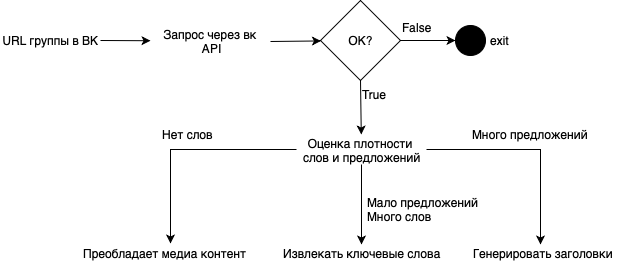
\includegraphics{images/app_story.png}
}

\caption{
\label{app_story} Принцип работы системы.
        }
\end {center}
\end {figure}

Рассмотрим теперь то, насколько актуальна данная проблема 
и какое место занимает предлагаемое решение среди существующих систем анализа
групп в социальных сетях.

На рынке уже существует большое множество сервисов дающих возможность проанализировать группу
на предмет возможного размещения рекламного поста \cite{smmpub2019}. Однако несмотря на
такое разнообразие сервисов, их функционал слабо отличается друг от друга. Как правило, предоставляется
возможность следить за аудиторией (ее полом, численностью, возрастом), частотой выпускаемого материала,
частотой выпуска материала и его типом. Однако никто из игроков не производит анализа содержания групп,
что кажется упущением возможности выделиться на рынке.

Наличие анализа содержания группы могло бы повысить скорость создания рекламы за счет уменьшения времени, необходимого для того, чтобы вникнуть в идею группы.

Причинами того, что создатели подобных сервисов не спешат с созданием таких услуг мы видим следующее:
\begin{itemize}
  \item Необходимо нанимать новых сотрудников, что влечет дополнительные расходы;
  \item Спрос на подобный функционал может быть низок из-за того, что в случае успеха подобного функционала, может снизиться спрос на специалистов в области SMM.
  \item Поскольку спрос низкий, то данное предложение не предлагается.
\end{itemize}

Имея ввиду причины отсутствия подобного функционала, мы считаем, что есть смысл создать его в виде
черной коробки, которую можно будет подключать к уже существующим сервисам. В этой черной коробке
использовать алгоритмы, которые показали отличные результаты на академических датасетах и рекомендовать их как базовые, однако оставить выбор за разработчиками при выборе алгоритмов.

Таким образом стоят следующие задачи:

\begin{itemize}
  \item Проанализировать существующие алгоритмы выделения ключевой информации из текстов;
  \item Предоставить возможность воспользоваться этими решениями как черным ящиком, создав интерфейсы для разработчиков:
  \begin{itemize}
    \item Библиотеку на python
    \item REST API, чтобы была возможность использовать из других языков программирования
  \end{itemize}
\end{itemize}

\section{Обзор литературы}
Задача сжатия текста с малой потерей смысла и сохранением возможности его прочтения
имеет название задачи \textit{суммаризации}. При этом, есть два концептуальных подхода к решению:
экстрактивный, когда для создания краткого содержания извлекаются целые куски текста вплоть до предложений,
и абстрактивная, где в кратком содержании могут быть слова, которых не было в исходном тексте.

В частности, при исследовании абстрактивной генерации заголовков, мы отталкивались от статьи Вконтакте, посвященной данной проблеме \cite{gavrilov2018self}. Ими предлагается применять нейронные сети с архитектурой Transformer и предобработкой Byte pair encoding (BPE) \cite{DBLP:journals/corr/SennrichHB15}. Однако в задаче абстрактивной генерации заголовков существуют дебаты на тему того, что использовать в качестве входа модели. Поскольку долгое время SOTA были модели с архитектурой encoder decoder, то было невозможно использовать длинные входные последовательности. Потому авторы статьи \cite{Putra2018IncorporatingTS} исследуют различные подходы по предварительному извлечению "Topic sentence", которое нейронная сеть должна дальше обработать. Это предложение, как говорят авторы, в идеальном случае, должна отвечать на 5W1H. Но достаточно ответов на "что, кто, когда".

% Для экстрактивной суммаризации чаще всего используют алгоритм TextRank \cite{TextrankOriginal}.
% TODO: Add more desctiption
% https://docplayer.ru/26752739-Vydelenie-klyuchevyh-slov-v-russkoyazychnyh-tekstah.html
% http://www.dialog-21.ru/media/3995/sandrikova.pdf
% YAKE
% https://repositorio.inesctec.pt/bitstream/123456789/7623/1/P-00N-NF5.pdf
% Браславский

% Извлечение ключевых слов

Несмотря на значительный прогрессы в различных областях за последние несколько лет, задача извлечения значимых \textit{ключевых слов} все еще не решена, поскольку эффективность существующих алгоритмов все еще далека от удовлетворительной в отличии от многих других ключевых областей computer science. Большинство традиционных подходов используют обучение с учителем, которое в значительной степени зависит от наличия доступа к размеченным данным для обучения. Один из первых подходов для выделения ключевых слов был предложен Turney \cite{Turney2000LearningAF}, который разработал специально разработанный алгоритм под названием GenEx.

Подавляющее большинство подходов, разработанных до сих пор основываются на обучении с учителем для выбора релевантных ключевых слов. Возможно, наиболее распространенной реализацией такого подхода является KEA \cite{Witten:1999:KPA:313238.313437}, который использует алгоритм Naive Bayes для извлечения ключевых слов. Несмотря на их часто превосходящую эффективность, основным ограничением алгоритмов обучения с учителем является их относительно длительный процесс обучения.

Это отличает алгоритмы обучения без учителя, которые могут быстро применяться к документам на разных языках или или из разных предметных областей и выдавать результат за короткий промежуток времени. В статье \cite{yake1, yake2} описывается YAKE, алгоритм извлечения ключевых слов, который основан на статистических признаках текста, извлеченных из одного документа, для идентификации и ранжирования наиболее важных ключевых слов. Ключевые аспекты YAKE! состоят в том, что не требуется обучение на конкретном наборе документов, и, следовательно, может быть легко применен к отдельным текстам, независимо от наличия корпуса, словаря или любой внешней коллекции. Алгоритм не использует ни извлечение именованных сущностей, ни разметку частей речи, что делает его независимым от языка, за исключением использования различных, но статических списков стоп-слов для каждого языка. Данные статьи являются оригинальными статьями по данному алгоритму и описывают принцип его работы, что является крайне необходимым для создания собственных реализаций.

Помимо YAKE, state of the art решениями в задаче извлечения ключевых слов все еще считается TextRank, графовый алгоритм экстрактивной суммаризации, который строит граф расстояний между токенами текста. Ключевой статьей при ознакомлении с работой данного алгоритма является оригинальная статья Рады и Тарау \cite{TextrankOriginal}. Данная статья

\section{Описание системы}

\section{Алгоритмы, использованные в работе}
Нами были использованы как классические подходы, так и новые, основанные на нейронных сетях.
В следующих секциях мы опишем их основные принципы, а также приведем ссылки на их реализации.

\subsection{Суммаризация текста}
Для суммаризации текста мы воспользовались алгоритмом экстрактивной суммаризации
основанном на TextRank \cite{DBLP:journals/corr/BarriosLAW16, rehurek_lrec, TextrankOriginal},
и моделью трансформера \cite{DBLP:journals/corr/VaswaniSPUJGKP17}, обученной на
датасете РИА новостей \cite{gavrilov2018self}.
Для предобработки данных модели трансформера мы использовали byte
pair encoding \cite{DBLP:journals/corr/SennrichHB15}.
Помимо этого мы извлекали первое предложение из новости.
Для TextRank и извлечения первого предложения не требуется обучающая выборка, что
делает их очень удобными в использовании. При этом, исследования показывают, что
в задаче генерации заголовков, первое предложение в новости --
это очень сильный бэйзлаин \cite{gavrilov2018self},
который трудно побить как экстрактивной, так и абстрактивной суммаризацией.

\subsubsection{Baseline}

В качестве бэйзлаина в задаче генерации заголовков используется первое предложение новости. Именно им мы и воспользовались и отталкивались от него.


\subsubsection{TextRank}

TextRank является является адаптацией идеи алгоритма PageRank \cite{Page98thepagerank} с задачи рекомендации страниц в интернете на задачу рекомендации лучшего предложения или набора слов в тексте. Сам алгоритм состоит в том, что мы текст превращаем в граф, где узлы -- это предложения, а для каждого ребра подсчитывается вес, где вес определяется по количеству совпавших слов в двух предложениях.

Таким образом, получается, что можно выбрать предложение с самыми тяжелыми ребрами в качестве предложения, которое описывало бы исходный текст.

\begin{figure}[ht]
\begin{center}

\scalebox{0.4}{
   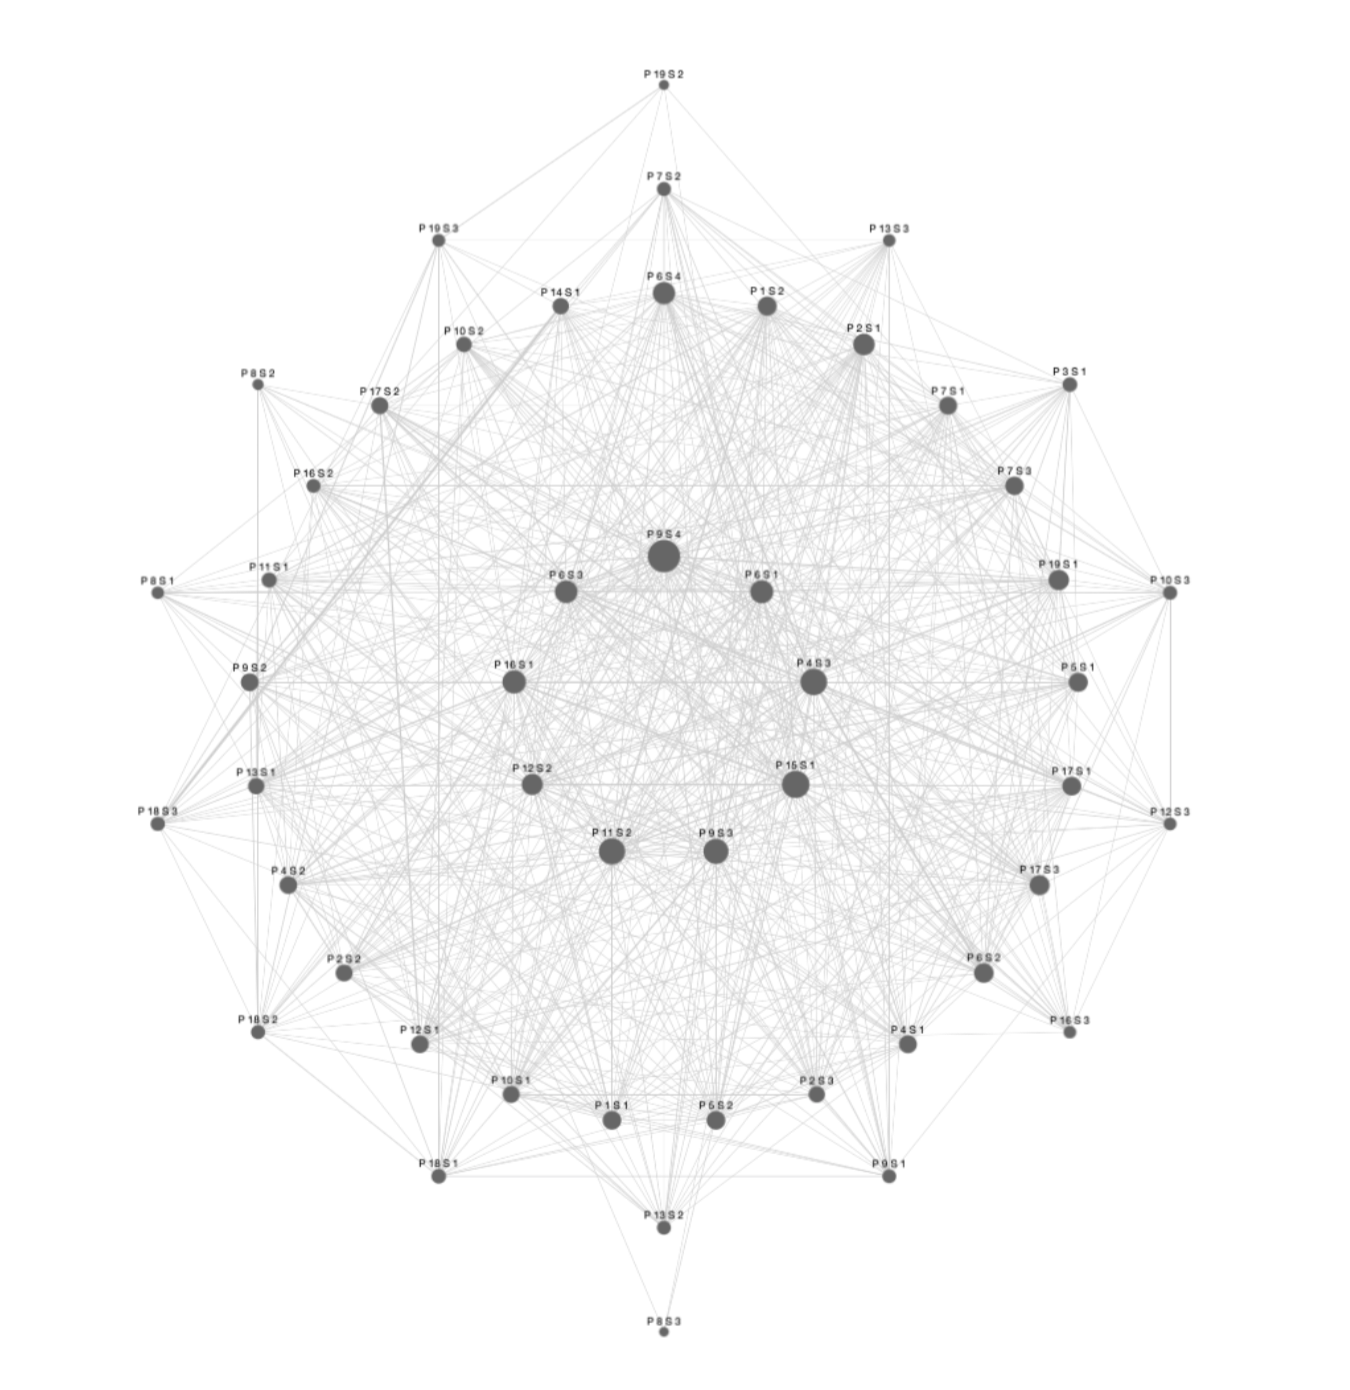
\includegraphics{images/text_rank_example_graph.png}
}

\caption{
\label{text_rank_example_graph}
        Пример результирующего графа textrank.}
\end {center}
\end {figure}

\subsubsection{Byte pair encoding}

Мы используем byte pair encoding (BPE), технику, предложенную Сеннрич для задачи машинного перевода в \cite{DBLP:journals/corr/SennrichHB15}. BPE -- это метод сжатия данных, в котором часто встречающиеся пары байтов заменяются дополнительными символами алфавита. В случае текстов, как в области машинного перевода, наиболее часто встречающиеся слова сохраняются в словаре, а менее часто встречающиеся слова заменяются последовательностью (обычно двумя) токенами. Например, для морфологически богатых языков окончания слов могут быть отделены, поскольку каждая форма слова определенно реже, чем ее основа. Кодирование BPE позволяет нам представлять все слова, включая те, что не встречаются по время обучения, с фиксированным словарным запасом.

% \subsubsection{Beam search}


\subsubsection{Universal transformer network}
В то время как рекуррентные нейронные сети могут быть легко использованы для определения модели Encoder-Decoder, тренировка таких моделей очень дорого с точки зрения вычислений. Другой недостаток состоит в том, что они используют только локальную информацию, опуская последовательность скрытых состояний H = {h1, ..., hN}. То есть любые два вектора из скрытого состояния hi и hj связаны с вычислениями j - i RNN, что затрудняет улавливание всех зависимостей в них из-за ограниченной емкости. Чтобы обучить богатую модель, которая изучила бы сложную текстовую структуру, мы должны определить модель, которая опирается на нелокальные зависимости в данных.
В этой работе мы принимаем архитектуру модели Universal Transformer \cite{}, которая является модифицированной версией Transformer \cite{}. Этот подход имеет несколько преимуществ по сравнению с RNN. Прежде всего, его можно тренировать параллельно. Кроме того, все входные векторы связаны друг с другом через механизм Attention. Это подразумевает, что архитектура Transformer учитывает нелокальные зависимости между токенами независимо от расстояния между ними, и, таким образом, она может выучить более сложное представление текста в статье, что оказывается необходимым для эффективного решения задачи суммаризации.

\subsection{Выделение ключевых слов}

Статья Boudin, Florian \cite{boudin:2016:COLINGDEMO} рассматривает наиболее сильные подходы к выделению ключевых слов.
И основная суть их статьи в том, что они предлагают реализации основных алгоритмов выделения ключевых слов, однако проблема,
с которой мы столкнулись состоит в том, что в ядре их библиотеки заложена библиотека spacy \cite{honnibal-johnson:2015:EMNLP}, которая не работает с русским языком
% Конкретно, они показывают для каких задач доходят какие алгоритмы. Основная таблица этой статьи приведена на таблице \ref{keywords_extraction_report},
% и она говорит о том, какие алгоритмы показывают лучшие результаты на каких задачах.

Таким образом, для данной работы мы реализовали TopicRank, TfIdf и YAKE и TextRank поскольку эти алгоритмы считаются лучшими алгоритмами для выделения ключевых слов. Мы выложили эти реализации в качестве библиотеки на python \footnote{https://github.com/imemedb/keyverbum}, реализовав интерфейсы библиотеки Scikit-Learn \cite{scikit-learn, sklearn_api}.

% \begin{table}[ht]
%   \begin{center}
%     \begin{tabular}{|l|l|l|l|l|}
%       \hline
%       \textbf{Dataset} & \textbf{Approach and System} & \textbf{P} & \textbf{R} & \textbf{F} \\ \hline
%       Абстракты & TopicRank & 35.0 & 66.0 & 45.7 \\ \hline
%       Блоги & CommunityCluster & 35.1 & 61.5 & 44.7 \\ \hline
%       Новости & \begin{tabular}[c]{@{}l@{}} TextRank \end{tabular} & 28.8 & 35.4 & 31.7 \\ \hline
%       Научные статьи & \begin{tabular}[c]{@{}l@{}}Statistical, semantic, \\ and distributional features\end{tabular} & 27.2 & 27.8 & 27.5 \\ \hline
%     \end{tabular}
%     \caption{
%       \label{keywords_extraction_report} Sate of the art результаты извлечения ключевых слов на классических датасетах. P -- точность, R -- полнота, F -- среднее гармоническое точности и полноты.
%     }
%   \end{center}
% \end{table}

\subsubsection{Keyverbum}
Написанная нами библиотека содержит в себе четыре популярных алгоритма выделения ключевых слов: TopicRank, TfIdf и YAKE и TextRank.
Для для того, чтобы их использовать в других проектах, связанных с машинным обучением, они были реализованы как наследники
ClassifierMixin, что означает, что у них должны быть реализованы методы fit и predict.

При этом, было принято решение вынести этап чистки данных и разбиение на токены за пределы экстракторов ключевых слов.
Таким образом, алгоритмы извлечения ключевых слов ожидают на вход уже готовый список токенов.

В результате, использование этих алгоритмов выглядит следующим образом:

\begin{verbatim}
from keyverbum.keywords import (Textrank, 
                                preprocessing_pipeline)

text = "some text"
prep_text = preprocessing_pipeline.transform(text)

extractor = Textrank(n_keywords=10)

keywords = extractor.fit_predict(prep_text)

\end{verbatim}

Помимо этого, был реализован REST API, который можно развернуть на своем сервере.
Таким данными алгоритмами можно воспользоваться в других приложениях, написанных не
только на Python.


\subsubsection{TopicRank}
TopicRank - это метод обучения без учителя, целью которого является извлечение ключевых фраз из наиболее важных тем документа. Темы определяются как кластеры похожих ключевых фраз-кандидатов. Извлечение ключевых фраз из документа состоит из следующих шагов, показанных на рисунке \ref{topicrank}. Во-первых, документ предварительно обрабатывается (сегментация предложений, разметка слов и тегирование частей речи), а кандидаты в ключевые фразы группируются по темам. Затем темы ранжируются в соответствии с их важностью в документе, и ключевые фразы извлекаются путем выбора одного кандидата ключевой фразы для каждой из наиболее важных тем.

\begin{figure}[ht]
\begin{center}

\scalebox{0.4}{
   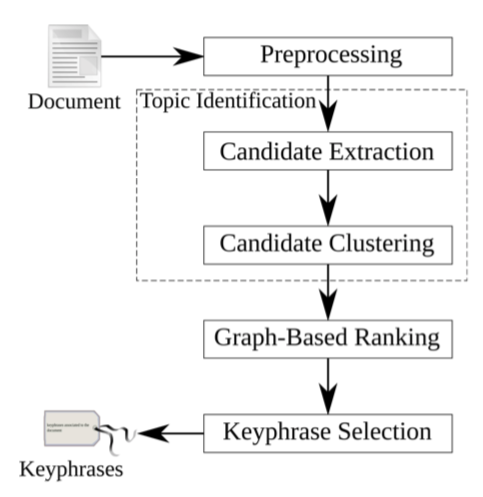
\includegraphics{images/how_topicrank_works.png}
}

\caption{
\label{topicrank}
        Принцип работы TopicRank.}
\end {center}
\end {figure}

% \subsection{Суммаризация изображений}
% Для суммаризации изображений мы реализовали алгоритм,
% описанный в статье \cite{DBLP:conf/icsipa/SharmaKASK15}.
% Основная идея состоит в том, что из изображений извлекаются
% признаки, инвариантные к поворотам \cite{Lowe:2004:DIF:993451.996342},
% эти признаки кластеризуют
% используя k-means \cite{Arthur:2007:KAC:1283383.1283494} и индексы кластеров
% используют как признаки для латентного размещения
% Дирихле \cite{Blei:2003:LDA:944919.944937, rehurek_lrec}.
%
% Помимо этого, мы попробовали
% на нашей задаче обучению метрике между изображениями
% \cite{DBLP:journals/corr/abs-1803-11095, DBLP:journals/corr/abs-1810-06951}.

\subsubsection{YAKE}
Алгоритм состоит из 6 основных этапов: предварительная обработка текста, извлечение признаков, индивидуальная оценка токенов, формирование списка ключевых слов кандидатов, дедупликация данных и ранжирование.

Сначала применяется предварительная обработка, которая разбивает текст на отдельные токены на основе пробела или специального символа (например, разрывы строк, скобки, запятая, точка и т. д.). Во-вторых, выделяется набор из пяти признаков, чтобы охватить характеристики каждого отдельного токена. Это регистр, позиция токена, частота токена, контекст токена и как часто токен появляется в различных предложениях.

Регистр учитывает то, написано ли слово с большой буквы.
Оценка позиции слова учитывает то, где находится слово в документе, исходя из предположения, что релевантные ключевые слова часто имеют тенденцию концентрироваться больше в начале документа. 
Частота слова указывает на то, как часто встречается слово в тексте. Четвертной признак, контекст токенов, вычисляет количество различных токенов, встречающихся с левой (или правой) стороны слова-кандидата. Чем больше количество различных токенов, которые встречаются со словом-кандидатом (с обеих сторон), тем более бессмысленным будет слово-кандидат. Наконец, частота токена в различных предложениях количественно определяет, как часто слово-кандидат встречается в разных предложениях. Подобно частоте слов, частота токена в различных предложениях больше ценит те слова, которые часто встречаются в разных предложениях. Оба признака, тем не менее, сочетаются со контекстом слов, что означает, что чем чаще они встречаются в разных предложениях, тем лучше, если они не встречаются часто с разными словами. 

На третьем этапе эти признаки  эвристически объединяются одной величиной, так что каждому токену присваивается величина $S(w)$. Эта величина будет принимать участие в  процессе генерации ключевых слов, который выполняется на четвертом шаге. Здесь мы рассмотрим скользящее окно из 3 граммов, таким образом генерируя непрерывную последовательность из 1, 2 и 3 граммов ключевых слов-кандидатов. Каждому ключевому слову-кандидату будет присвоен окончательный $S(kw)$, так что чем меньше оценка, тем более значимым будет ключевое слово. Уравнение 1 описывает это:

\begin{equation}
    S(kw) = \frac{\prod_{w \in kw}{S(w)}}{TF(kw)*(1+\sum_{w\in kw}{S(w)})}
\end{equation}

где $S(kw)$ - оценка ключевого слова-кандидата, определяемая путем умножения (в числителе) оценки $S(w)$ первого члена ключевого слова-кандидата на последующие оценки оставшихся токенов. Результат делится на сумму оценок $S(w)$ для усреднения по длине ключевого слова, так что более длинные n-граммы не получают выгоды только потому, что они имеют более высокое $n$. Результат далее делится на $TF(kw)$ - частоту использования ключевого слова - для уменьшения влияния менее частых кандидатов. На пятом этапе исключается аналогичные кандидаты из предыдущих шагов. Для этого используется расстояние Левенштейна \cite{Levenshtein_SPD66}. Наконец, система выведет список релевантных ключевых слов, составленный из 1, 2, 3 грамм, так что чем ниже показатель S(kw), тем более важным будет ключевое слово.


\subsection{Оценки качества}
Для оценки качества выделения ключевых слов мы использовали среднюю абсолютную точность $P$, полнту $R$ и их среднее гармоническое $F1$.
Данные метрики являются стандартными при оценке качества моделей выделения ключевых слов.
Формулы их рассчета приведены ниже, а их реализацию можно найти в нашей библиотеке keyverbum \footnote{https://github.com/imemedb/keyverbum/blob/master/keyverbum/evaluate.py}

\begin{equation}\label{eq:prf1}
    P_{i} = \frac{tp}{tp + fp} \quad R_{i} = \frac{tp}{tp + fn} \quad F1_{i}=2\frac{P_{i}*R_{i}}{P_{i}+R_{i}}
\end{equation}

На управлениях \ref{eq:prf1} $tp$, $fp$, $fn$ обозначают количество правильно выбранных ключевых слов, ложно правильно выбранных ключевых слов и ложно неправильно, соответственно.
При этом, $P_i$, $R_i$ и $F1_i$ считаются для каждого примера, и имея эти метрики для каждого примера, в результате считается среднее.

Для оценки качества моделей генерации заголовков мы использовали метрику ROUGE-1, 2, L $P$, $R$, $F1$ \cite{Lin:2004}, где 1, 2, L обозначают рамер использованных
n-грамм, а $P$, $R$, $F1$ -- это точность, полнота и их среднее гармоническое, почитанные по формулам \ref{eq:rougepf}. В этих формулах $number\_of\_overlaping\_words$ -- это количество n-грамм, которые совпадают в предсказании и истинном заголовке, $total\_words\_in\_reference$ -- это количество n-грамм в истинном заголовке, а $total\_words\_in\_prediction$ -- это количество n-грамм в предсказнном заголовке.

\begin{equation}\label{eq:rougepf}
\begin{gathered}
P = \frac{number\_of\_overlaping\_words}{total\_words\_in\_reference} \\ 
R = \frac{number\_of\_overlaping\_words}{total\_words\_in\_prediction}
\end{gathered}
\end{equation}

Разберем на конкретном примере, как используются эти метрики. Представим, что истинным текстом является "кошка была найдена под кроватью", а некоторым предсказанием является "кошка под кроватью".
Тогда для 1-грамм, точность или ROUGE-1 $P$ = $\frac{3}{5}$ = $0.6$, а полнота или ROUGE-1 $R$ = $\frac{3}{3}$ = $1.0$.

В случае ROUGE-2 в качестве токенов берутся последовательно биграммы, а при подсчете ROUGE-L количество пересекающихся токенов заменяется на поиск длинны максимальной подпоследовательности и точность и полнота тогда считаются по формуле \ref{eq:rougelpf}, где $LCS$ -- длинна самой динной пересекающейся подпоследовательности.

\begin{equation}\label{eq:rougelpf}
\begin{gathered}
P = \frac{LCS(reference, prediction)}{total\_words\_in\_reference} \\ 
R = \frac{LCS(reference, prediction)}{total\_words\_in\_prediction}
\end{gathered}
\end{equation}

Оценка алгоритмов генерции заголовков, с использованием данных метрик, производилась на датасете 
РИА новостей \cite{gavrilov2018self}. Помимо этого,
на основе этого датасета проводилось соревнование по генерации заголовков, где автором было
получено 3 место, а описание результатов соревнования было принято в качестве статьи на конференцию "Диалог".

% Помимо этого, как для текстовых данных, так и для изображений, мы  использовали
% Яндекс.Толоку \cite{yandex_toloka_2019}, чтобы привлечь людей к оценке качества наших результатов.


\section{Анализ использованных данных}
% Рассказать про датасет Риа новостей и данные из ВК.

В работе были использованы несколько датасетов с целью выбора алгоритмов под соответствующие задачи.
В частности, мы воспользовались датасетом оценки качества выделения ключевых слов \cite{mannefedov2019}, недавно
опубликованным датасетом Риа новостей \cite{gavrilov2018self}, а также в нашей работе мы используем
данные из 25 групп вконтакте с разным целевым материалом: от медиа контента до полноценных длинных
текстов.

\subsection{Данные выделения ключевых слов}

\begin{table}[ht]
  \begin{center}
    \begin{tabular}{|l|l|l|l|}
      \hline
      \textbf{Датасет} & \textbf{Тип} & \textbf{\begin{tabular}[c]{@{}l@{}}Количество \\ документов\end{tabular}} & \textbf{\begin{tabular}[c]{@{}l@{}}Среднее \\ количество \\ токенов\end{tabular}} \\ \hline
      Киберленика & Абстракты & 4072 & 5.27 \\ \hline
      Habr & Блоги & 3990 & 5.03 \\ \hline
      Независимая газета & Новости & 1987 & 6.11 \\ \hline
      Россия сегодня & Новости & 7217 & 10.07 \\ \hline
    \end{tabular}
  \end{center}
\end{table}

Для анализа качества использованных алгоритмов для выделения ключевых слов
мы воспользовались датасетом с разнообразными статьями на русском языке \cite{mannefedov2019}.
В наборе присутствуют научные статьи из "журнала киберленика" \cite{cyberlenica},
технического блога "хабрахабр" \cite{habr} и новостных ресурсов "Независимая газета" \cite{independentjournal} и "Россия сегодня" \cite{rt}.

% Таким образом, мы приводим русскоязычные аналоги всем англоязычным ресурсам из таблицы \ref{keywords_extraction_report}.

\subsection{Данные для генерации заголовков}

Для обучения и выбора алгоритмов генерации заголовков, мы воспользовались недавно опубликованным
датасетом Риа новостей. Этот датасет содержит новости с января 2010 по декабрь 2014.
В нем имеется 1003869 новостных статей со средним размером заголовка 9.5 слов и
средней длинной текста 315.6 слов.

Эти датасет предоставлен в виде необработанных фрагментов оригинальных html-страниц.
Это означает, что в данных присутствовали различные HTML-теги и объекты.
В итоге имеется необработанная новость и соответствующий заголовок.

\begin{verbatim}

<p> <strong> <\strong> <\p> \n <p> <strong> Moscow,
Dec 1 &nbsp; &mdash; RIA news. <\strong> a fire in &nbsp;
one of the &nbsp; workshops in &nbsp;...<\p>
\end{verbatim}

В результате первым делом мы попытались очистить данные от ненужной информации. И так, мы создали препроцессор, который удаляет все html-теги и сущности.

Кроме того, мы обнаружили, что иногда в данных отсутствует текст, поскольку исходные новости представлены в виде изображений (например, снимок экрана Twitter), а новости чисто польские. Это все выбросы, с которых мы очистили данные.


\section{Эксперименты}
В данной секции мы приводим технические детали, параметры моделей и оценки качества созданных моделей на датасетах описанных выше.

\subsection{Генерация заголовка}
На практике обычно используется метрика ROUGE \cite{Lin:2004} при оценке качества алгоритмов суммаризации. Конкретно используются так называемые ROUGE 1,2, L - точность, полнота и F1. Имена в ROUGE X - Y обозначают следующее: X - количество n-грамм, используемых для вычисления метрики Y. В случае n-грамм размера L рассматривается самая длинная общая подпоследовательность из предсказанной последовательности найденая в исходной последовательности. Метрики Y - классическая точность, полнота и их среднее гармоническое.

В случае алгоритма Textrank \cite{DBLP:journals/corr/BarriosLAW16}, алгоритма экстрактивной суммаризации, мы воспользовались реализацией из библиотеки gensim \cite{rehurek_lrec}. В случае этого алгоритма, выделяется не одно предложение, а подмножество текста определенного размера, потому мы установли параметр отвечающий за размер возвращаемого текста равным 20\% от исходного.

Мы взяли state of the art реализацию алгоритма Universal Transformer из Open NMT \cite{2017opennmt} и обучили этот алгоритм на данных Риа новостей. Мы использовали 4 слоя кодировщика и декодеривщика, 8 heads of attention, вероятность дропаута была выставлена равной 0.3. Для оптимизации был использован алгоритм Adam с изменяющейся скоростью обучения, по правилу из оригинальной статьи о трансформере.

В качестве входа модели мы использовали первые 2000 BPE токенов.

Что касается обучения Byte Pair Encoder, то мы попробовали пердобученный на википедии токенизатор и обученный на датасете Риа новостей. В таблице \ref{headline_gen_results} они обозначены Wiki BPE и Ria BPE, соответственно.

Также для отбора лучших кандидатов для заголовка мы использовали beam search размером 10.

\begin{table}[htbp]
  \small
  \centering
  \begin{tabular}{|l|l|l|l|l|l|l|l|l|l|}
    \hline
    Algorithm\textbackslash{}Score                                                             & 1F   & 1P   & 1R   & 2F   & 2P   & 2R   & LF   & LP   & LR   \\ \hline
    First sentence                                                                             & 0.23 & 0.16 & 0.44 & 0.10 & 0.07 & 0.21 & 0.16 & 0.15 & 0.40 \\ \hline
    \begin{tabular}[c]{@{}l@{}}Wiki BPE \\ transformer\end{tabular}& 0.37 & 0.39 & 0.36 & 0.20 & 0.21 & 0.19 & 0.34 & 0.37 & 0.34 \\ \hline
    % \begin{tabular}[c]{@{}l@{}}Wiki BPE transformer\\ (first sentence, beam=5)\end{tabular} & 0.39 & 0.41 & 0.39 & 0.22 & 0.23 & 0.22 & 0.37 & 0.39 & 0.37 \\ \hline
    % \begin{tabular}[c]{@{}l@{}}Wiki BPE \\ transformer\\ (first sentence, beam=1)\end{tabular} & 0.37 & 0.37 & 0.37 & 0.20 & 0.20 & 0.20 & 0.34 & 0.36 & 0.35 \\ \hline
    \begin{tabular}[c]{@{}l@{}}Ria BPE \\ transformer\end{tabular}       & 0.36 & 0.37 & 0.35 & 0.18 & 0.20 & 0.18 & 0.33 & 0.36 & 0.33 \\ \hline
    \begin{tabular}[c]{@{}l@{}}Textrank \\ summarization\end{tabular}                          & 0.14 & 0.09 & 0.41 & 0.05 & 0.03 & 0.17 & 0.09 & 0.08 & 0.38 \\ \hline
    % \begin{tabular}[c]{@{}l@{}}Textrank keywords\end{tabular}                                & 0.09 & 0.07 & 0.18 & 0.00 & 0.00 & 0.01 & 0.05 & 0.05 & 0.14 \\ \hline
    \end{tabular}
  \caption{
  \label{headline_gen_results}
  ROUGE-1,2,F1, precision and recall scores.
  }
\end{table}

\begin{table}[htbp]
\scriptsize
\centering
\begin{tabular}{|l|l|}
\hline
Score & Example \\ \hline
0.00 & \begin{tabular}[c]{@{}l@{}}\textbf{Text}: 8 декабря 1991 года россия, белоруссия и украина подписали соглашение\\о создании содружества независимых государств (снг).\\ \textbf{Ground truth}: встреча в беловежской пуще\\ \textbf{Prediction}: заявил\end{tabular} \\ \hline
0.00 & \begin{tabular}[c]{@{}l@{}}\textbf{Text}: более 70 международных художников и арт-групп примут участие в основном\\проекте "больше света" \\ 5-й московской биеннале современного искусства,который будет показан в цвз "манеж" \\ с 20 сентября по 20 октября, сообщили риа новости в пресс-службе проекта.\\ \textbf{Ground truth}: стали известны все участники основного проекта\\5-й московской биеннале\\ \textbf{Prediction}: более 00 художников представят проект "больше света" в "манеже"\end{tabular} \\ \hline
0.99 & \begin{tabular}[c]{@{}l@{}}\textbf{Text}: фонд "сколково" и корпорация intel подписали в четверг соглашение\\о сотрудничестве, передает корреспондент риа новости.\\ \textbf{Ground truth}: "сколково" и intel подписали соглашение о сотрудничестве\\ \textbf{Prediction}: "сколково" и intel подписали соглашение о сотрудничестве\end{tabular} \\ \hline
\end{tabular}
\caption{
  \label{headlie_get_examples}
  Лучшие и худшие результаты предсказания модели. Score среднее от ROUGE-1,2,L F1.
  }
\end{table}

В Таблице \ref{headlie_get_examples} среднее от ROUGE-1,2, L F1 используется в качестве метрики. Мы показываем два примера: лучшее и худшее возможное предсказание нашего лучшего алгоритма -- Wiki transformer-а.

\subsection{Выделение ключевых слов}

Как видно из Таблицы \ref{mae_mean_kw}, лучшие результаты показывает TfIdf.

\begin{table}[ht]
  \begin{center}
    \begin{tabular}{l|lll|lll|lll|lll}
      \hline
      Датасет   &  \multicolumn{3}{|c|}{Независимая газета}      & \multicolumn{3}{|c|}{Россия Сегодня}       & \multicolumn{3}{|c|}{Habr}          \\
      \hline
      Алгоритм  &          P &            R &         F1 &          P &              R &         F1 &          P &       R &         F1 \\
          TfIdf &       0.13 &         0.07 &       0.08 &       0.08 &           0.08 &       0.08 &       0.16 &    0.08 &       0.10 \\
      TopicRank &       0.05 &         0.02 &       0.03 &       0.03 &           0.03 &       0.03 &       0.05 &    0.02 &       0.03 \\
       TextRank &       0.09 &         0.04 &       0.06 &       0.06 &           0.06 &       0.06 &       0.12 &     0.6 &       0.07 \\
           YAKE &       0.06 &         0.03 &       0.04 &       0.05 &           0.05 &       0.04 &       0.13 &    0.06 &       0.08 \\
      \hline
    \end{tabular}
    \caption{
      \label{mae_mean_kw} Средняя абсолютная точность (P), полнота (R), и F1 мера.
    }
  \end{center}
\end{table}


% У заключения нет номера главы
\section*{Заключение}
В данной работе мы предложили решение задачи краткого описания новостного ресурса. Решение включает в себя путь того, как с этой системой будет взаимодействовать пользователь, техническую архитектуру системы, обоснование выбранных алгоритмов, отталкиваясь от соответствующих решаемых подзадач.

% Убрать графическую часть
Как результат, с алгоритмической точки зрения, система была разбита на две подзадачи: выделения ключевых слов и генерации заголовков. Нами были предложены лучшие алгоритмы, для решения соответствующих задач. Также в этой работе мы заложили фундамент для дальнейших исследований в этой области, предоставив интерфейс для разработчиков и людей.

\setmonofont[Mapping=tex-text]{CMU Typewriter Text}
\bibliographystyle{ugost2008ls}
\bibliography{diploma.bib}
\end{document}
